\documentclass[10pt]{article}

\usepackage{fullpage}
\usepackage{graphicx}
\usepackage{mathtools}
\usepackage{setspace}
\usepackage{mdwlist}
\usepackage[center]{caption}
\onehalfspacing

\begin{document}
\title{Project Proposal\\Augmented Reality Image Processing System}
\author{Logan P. Williams \& Jos\'{e} E. Cruz Serrall\'{e}s}
\date{November 15, 2011}
\maketitle

\section*{Abstract}
We will implement an augmented reality system that can overlay a digital image on video of a real world environment. We read NTSC video from a video camera and store it in ZBT SRAM. A picture frame with colored markers on the corners is held in front of the camera. We then perform chroma-based object recognition to locate the coordinates of the corners. Using these coordinates, we apply a low-pass filter and a projective transformation to project an image onto the dimensions of the picture frame. We then output VGA video of the original captured image, with the processed image overlayed on top of the frame.

<<<<<<< HEAD
<<<<<<< HEAD
\tableofcontents
\newpage

\section{Introduction}

The augmented reality image processing system has six primary modules. The {\tt memory\_interface} module handles reading and writing from the ZBT memory, so that it can be abstracted away from the other modules. Raw video is read from the video camera by the {\tt ntsc\_capture} module, which also finds pixels that match the colors on the corners of the frame. These pixels are read by the {\tt object\_recognition} module which finds the center of mass of the frame corners, and calculates the downsampling coefficients in each direction. The {\tt LPF} module performs the low pass filtering in two stages, described in detail below. On the second stage, it sends each pixel ``on-the-fly'' to the {\tt projective\_transform} module which then sends that pixel's new coordinates to the {\tt memory\_interface} module to be written. The {\tt vga\_write} module reads and transmits the VGA data to be generated by the video DAC.
=======
% \tableofcontents
>>>>>>> 4f1e49314170ebf0d7282a6d0144125322e4ee8b
=======
% \tableofcontents
>>>>>>> 4f1e49314170ebf0d7282a6d0144125322e4ee8b

\begin{figure}[h!]
\centering
<<<<<<< HEAD
<<<<<<< HEAD
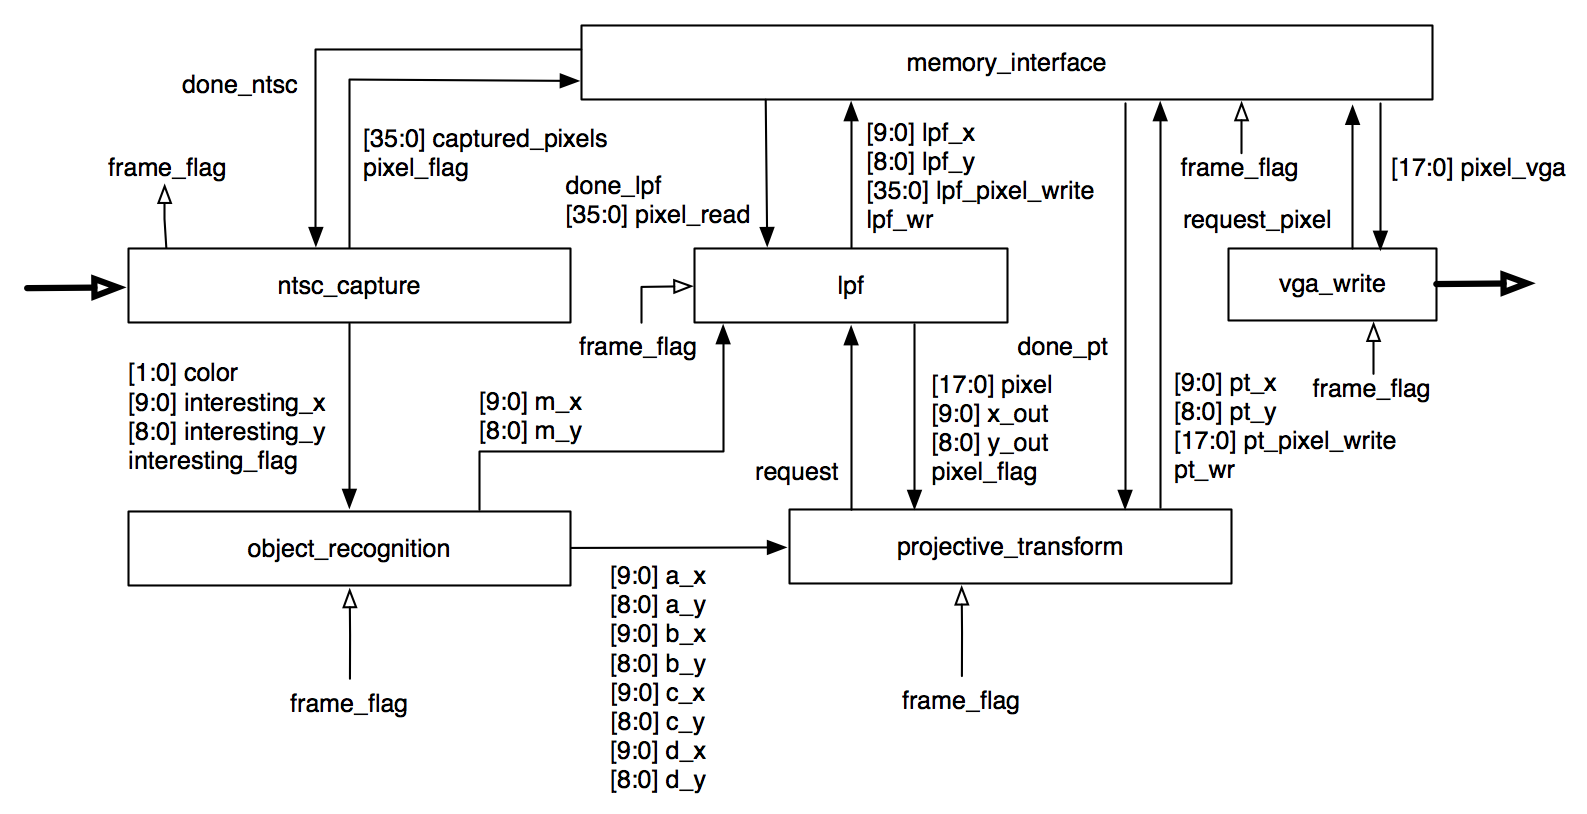
\includegraphics[width=\textwidth]{block_diagram_with_wires.png}
\caption{\emph{Augmented reality image processing system.}}
=======
=======
>>>>>>> 4f1e49314170ebf0d7282a6d0144125322e4ee8b
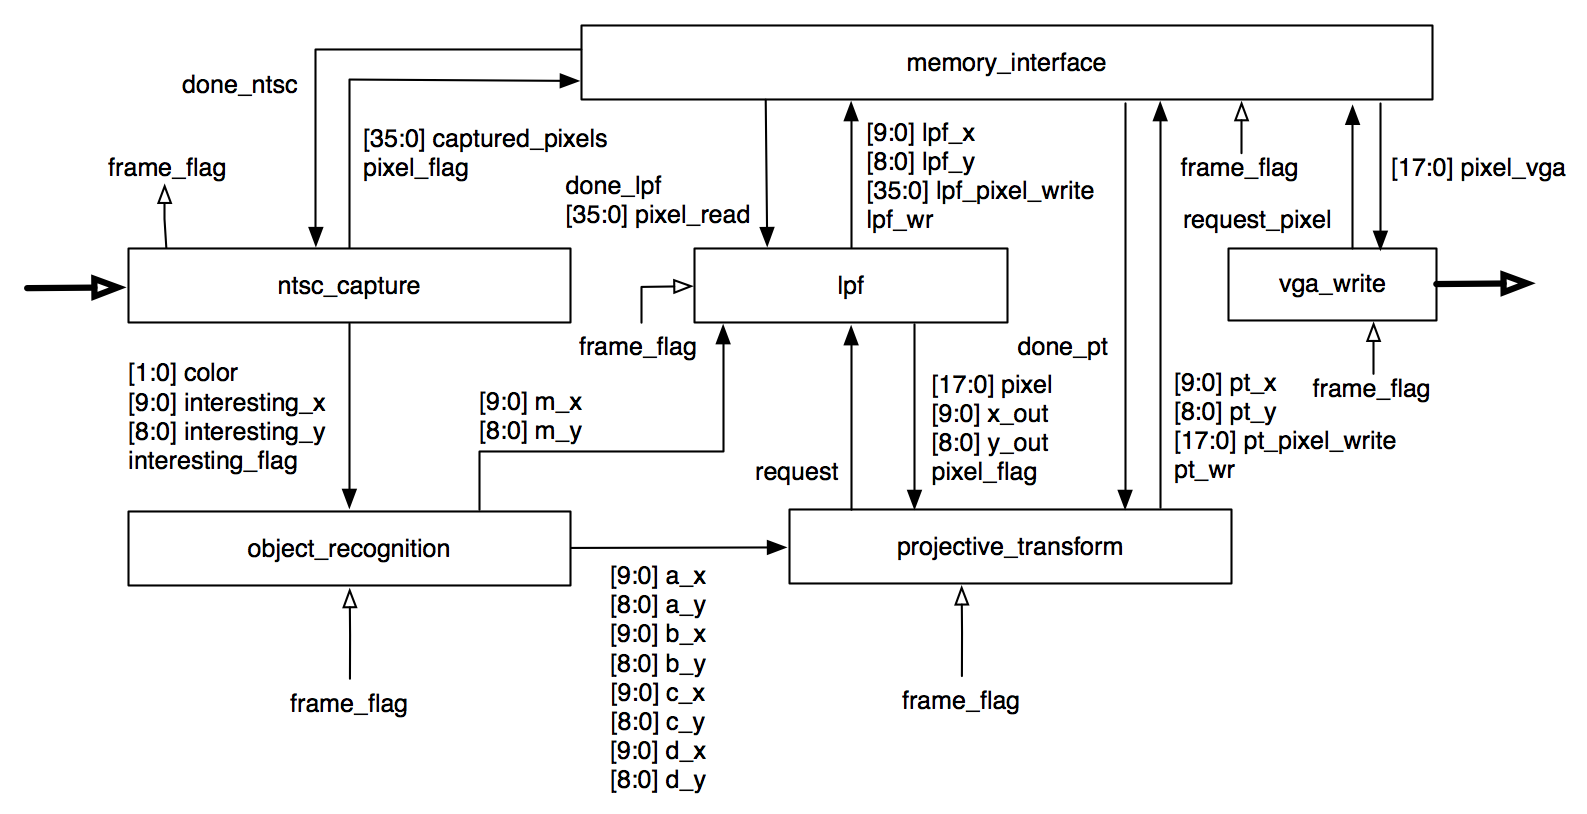
\includegraphics[width=0.8\textwidth]{block_diagram_with_wires.png}
\caption{\emph{The block diagram of the augmented reality system.}}
>>>>>>> 4f1e49314170ebf0d7282a6d0144125322e4ee8b
\end{figure}
\section{Submodules}
% 1) inputs & outputs
% 2) some indication of its complexity and level of performance
%	a) number and type of arithmetic operations
%	b) size of internal memories
%	c) required throughput
%	etc.
% 3) how the module will be tested
% 4) who will be writing the module
\subsection{{\tt ntsc\_capture} (Logan)}
The {\tt ntsc\_capture} module decodes NTSC Composite video using an Analog Devices ADV7185 video ADC and sends pixels in luminance/chrominance color space to {\tt memory\_interface} to be written into a ZBT memory frame buffer.

Additionally, when the {\tt ntsc\_capture} module sees a color that matches the target (blue, green, red, and yellow), it sends the color and the X/Y location of the pixel to the {\tt object\_recognition} module. It also sends a flag that goes high when the entire frame has been captured, and a new one is beginning. The exact names of these outputs, and of every input/output described below can be seen on the block diagram above.

This module can be tested by connecting it to the {\tt vga\_write} module and ensuring that the video output is the image seen by the video camera.

\subsection{{\tt memory\_interface} (Jos\'{e})}
% Jose
The {\tt memory\_interface} module handles the interaction between all of the other modules and the two ZBT Memory blocks, which house the four images that the modules use for capturing, displaying, and processing. Ideally, BRAM would have been used, but the number of pixels that we would like to store vastly exceeds BRAM capacity. Unlike BRAM, each ZBT Memory block can only handle one read or write operation per cycle, causing memory access to be the main bottleneck of our system. As such, we will store only the six most significant bits of each component of every pixel, allowing us to store two pixels per address and to reduce the number of memory accesses in our system by a factor of two. The number of required memory acceses per module and the distribution of the images in the RAM necessitates a minimum clock frequency of 50.7MHz, which is reasonable given the propagation delays of multipliers and other elements.

{\tt memory\_interface} will allocate two images per memory block. These four images will be (1) {\it capture}, the image being captured from NTSC; (2) {\it display}, the image being displayed in the VGA; (3) {\it processing}, the image that will be processed by {\tt LPF} and projected by {\tt projective\_transform}; and (4) {\it next\_display}, the image to which {\tt projective\_transform} will write and the next image that will be displayed. Every image refresh (1/30 seconds), the previous {\it next\_display}, {\it display}, {\it capture}, and {\it processing} image locations will become the next {\it display}, {\it processing}, {\it next\_display}, and {\it capture} image locations, respectively. These location shifts will be transparent to the other modules. Read and write requests from {\tt vga\_write} and {\tt ntsc\_capture} will be given priority over requests from other modules.

The inputs to {\tt memory\_interface} are (1) frame\_flag, which signals when to shift; (2) two pixels from {\tt ntsc\_capture}; (3) two (x,y) pairs, one from {\tt LPF} and one from {\tt projective\_transform}; (4) two pixels from {\tt LPF}; (5) one pixel from {\tt projective\_transform}; and (6) request flags and (7) write flags from other submodules. The outputs from {\tt memory\_interface} are (1) done flags; (2) one pixel to {\tt vga\_write}; and (3) two pixels to {\tt LPF}.

{\tt memory\_interface} will be tested in stages. Initially, basic read and write functionality will be assessed in simulation and then on the FPGA. Once we have written and read information from the ZBT RAM successfully, we will attempt to write, read, and display an image. Finally, all of the logic pertaining to handling read and write requests from all the modules simulatenously will be written, tested using extensive testbenches, and finally tested on an FPGA with dummy modules. All of this testing should avoid help us avoid headaches during final integration.

\subsection{{\tt object\_recognition} (Logan)}
The {\tt object\_recognition} module collects ``interesting'' pixels located by the NTSC Capture module, and calculates the center of mass of each color, to find the location of the corners of the picture frame.

It takes as inputs (1) the color of a detected pixel, (2) a flag that goes high for one clock cycle when a pixel is detected, (3) the X/Y coordinates of the pixel, and (4) a flag that goes high when a new frame is beginning. It produces as output four sets of X/Y coordinates, one for the center of mass of each color.

The center of mass will be calculating with a simple linear weighting scheme, averaging the X and the Y coordinate for each pixel independently to find the center X/Y location, which are used by the {\tt LPF} and the {\tt projective\_transfom} module. This module can be tested with a simple test bench that provides some sample pixel locations, and tests to see if the module computes the center of mass correctly.

\subsection{{\tt LPF} (Jos\'{e})}
The {\tt LPF} module's sole purpose is to apply a lowpass filter (LPF) to the {\it processing} image so as to avoid aliasing when {\tt projective\_transform} skews the image. The following steps detail the operation of {\tt LPF} every image refresh cycle (1/30 seconds): (1) Load the filter coefficients of a 1D LPF with cutoff frequency \( \frac{\pi}{M_y} \). (2) Apply this filter to each column of {\it processing} and store each column once again in {\it processing}. (3) Load the filter coefficients of a 1D LPF with cutoff frequency \( \frac{\pi}{M_x} \). (4) Apply this filter to each row of {\it processing} but instead feed the output pixels to {\tt projective\_transform}. (5) Wait for the next cycle. The image data will be buffered in BRAM, such that LPF accesses memory 1.5 times per pixel.

The inputs to {\tt LPF} are (1) \( M_x \) and (2) \( M_y \), the downsampling coefficients; (3) frame\_flag, which signals when to start filtering; (4) the done pulse and (5) the pixels from {\tt memory\_interface}; and (5) the request from {projective\_transform}. The outputs from {\tt LPF} to {\tt memory\_interface} are (1) the write signal, (2) the pixels to be written, and the (3) (x,y) coordinates of the leftmost written pixel. The outputs from {\tt LPF} to {\tt projective\_transform} are (1) the pixel flag, which signals when a new pixel is available; (2) the (x,y) coordinates of this new pixel; and (3) the new pixel.

The lowpass filters that will be used will be finite impulse response (FIR) Parks-McClellan filters. Most of the information contained in an image is contained in its phase. FIR filters were chosen because they can be made so as to have no effect on the phase of the image, preserving most of the information. Parks-McClellan filters were chosen because they are highly adaptable and easily calculated with MATLAB. The filter coefficients will be stored in BRAM for easy access. Because {\tt FIR} will only be filtering the luminance component of each pixel, the order, \( N \), of these filters will only be constrained by the number of multipliers on the FPGA and the number of multipliers used in other modules. The symmetry of these filters will be exploited, requiring only \( \frac{N}{2}+1 \) multiplications per pixel. We are aiming for filters of order 100, though filters of order 50 or greater will suffice.

Because {\tt LPF} is used only to make the output look nice, {\tt LPF} will be delegated to the end of the project. Given enough time, this module will be written and tested extensively with progressively more complicated testbenches. The initial testbench will apply to filter to an image with one white pixel, with all cutoff coefficients. The outputs of this testbench should match the coefficients in the BRAM. Once the module passes these tests, {\tt LPF} will be used on more complicated images, and the output will be compared to the ideal output with MATLAB. In these testbenches, different memory access cases will be tested, as well.

\subsection{{\tt projective\_transform} (Logan)}
% Logan
The inputs to {\tt projective\_transform} are (1) the pixel value last produced by {\tt LPF}, (2) a flag signal held high for one clock signal when {\tt LPF} has processed a new pixel, (3) the four coordinates of the corners of the frame provided by the {\tt object\_recognition} module, and (4) a signal when a new frame is beginning.

The outputs from {\tt projective\_transform} are (1) a request to {\tt LPF} for a new pixel, (2) the X/Y coordinates of the transformed pixel, (3) the transformed pixel value, and (4) a flag indicating that a new pixel is to be written.

This function maps the original rectangular image to any convex quadrilateral, provided that all sides of the destination quadrilateral are shorter than the original, which is inherent in the overall system. A graphic representation of the transformation is shown in Figure 2.

\begin{figure}[h!]
\centering
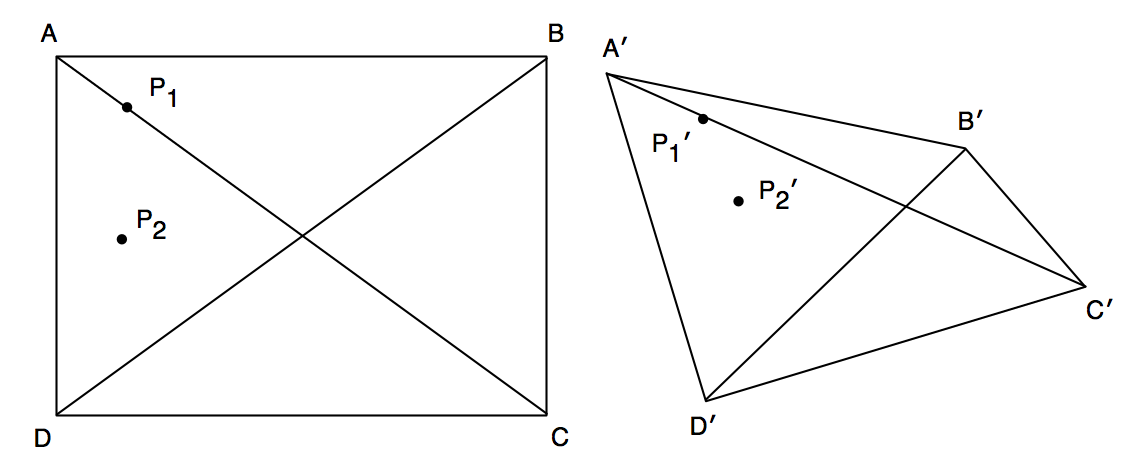
\includegraphics[width=0.65\textwidth]{arbiskew_graphic.png}
\caption{\emph{A visual representation of the result of the {\tt projective\_transform} module. Input is on the left, a possible output, for four coordinates $A\prime$, $B\prime$, $C\prime$, and $D\prime$ is on the right.}}
\end{figure}

Mathematically, the algorithm works as follows:
\begin{enumerate*}
\item Calculate the distance of line $\overline{A\prime D\prime}$ and assign it to $d_{ad}$.
\item Do the same for $\overline{B\prime C\prime}$ and assign it to $d_{bc}$.
\item Create two ``iterator points,'' point $I_A$ and $I_B$ initially located at $A\prime$ and $B\prime$.
\item Let $o_x = 0$ and $o_y = 0$
\item Calculate the distance between the iterator points, assign it to $d_i$.
\item Create a third iterator point, $I_C$ at the location $I_A$.
\item Assign the pixel value of $I_C$ to pixel $(o_x, o_y)$ in the original image.
\item Move $I_C$ along line $\overline{I_A I_B}$ by an amount $= \frac{d_i}{width_{original}}$.
\item Increment $o_x$.
\item Repeat steps 7--9 until $I_C = I_B$.
\item Move $I_A$ along line $\overline{A\prime D\prime}$ by an amount $= \frac{d_{ad}}{height_{original}}$.
\item Move $I_B$ along line $\overline{B\prime C\prime}$ by an amount $= \frac{d_{bc}}{height_{original}}$.
\item Increment $o_y$.
\item Repeat steps 5--13 until $I_A = D\prime$ and $I_B = C\prime$.
\end{enumerate*}

This algorithm needs a relatively small number of multiplications: two per pixel in the original image ($2\times640\times480$), and four per line in the original image ($4\times480$). There is also a square root required once per line, that will be implemented using a standard iterative algorithm.

The {\tt projective\_transform} module can be tested by creating a test bench that provides a series of test pixels as input. The output generated in ModelSim by {\tt projective\_transform} can then be compared with the output generated by a MATLAB implementation of the algorithm described above.

\subsection{{\tt vga\_write} (Jos\'{e})}
% Jose
The {\tt vga\_write} section is straightforward and will basically be a clone of the VGA code used in Lab 2 (Pong). Essentially, the output will be refreshed at a rate of 60Hz and output at a resolution of 640x480 pixels. This module will read the pixel values from displayed image and assign it based on the {\it hcount} and {\tt vcount} variables, which will be incremented accordingly. The clock signal used for this module will be synthesized with the ISE's toolkit. This module will be tested by loading a standardized image to memory and verifying whether {\tt vga\_write} displays this image properly on the monitor.

\section{External Components}
We will be using two standard external components: a video camera that provides NTSC composite video out, to be provided by the 6.111 staff, and a VGA display, available in the 6.111 lab.

\section{Project Deadlines}
% A calendar-like view of what deadlines we'll set ourselves, when everything should be operational, etc. Maybe this could be collapsed into the submodules section
<<<<<<< HEAD
<<<<<<< HEAD
\begin{itemize}
\item[] 11-11-2011 - Finalized Block Diagram
\item[] 11-18-2011 - First draft of ArbiLPF, ArbiSkew, and ZBT Memory written
\item[] 11-22-2011 - VGA Write and NTSC Capture first drafts written; ArbiLPF, ArbiSKEW, ZBT Memory fully tested
\item[] 11-30-2011 - NTSC Capture and VGA Write fully tested; start of full integration
\item[] 12-05-2011 - Full integration
\item[] 12-12-2011 - Final report due
\end{itemize}
=======
=======
>>>>>>> 4f1e49314170ebf0d7282a6d0144125322e4ee8b
\begin{description}
\item[11-11-2011] Finalized Block Diagram
\item[11-18-2011] First drafts of {\tt projective\_transform} and {\tt memory\_interface} written
\item[11-22-2011] First drafts of {\tt object\_recognition}, {\tt LPF}, {\tt vga\_write}, and {\tt ntsc\_capture} first drafts written; {\tt projective\_transform} and {\tt memory\_interface} fully tested
\item[11-28-2011] {\tt ntsc\_capture} and {vga\_write} fully tested; start of basic integration
\item[11-31-2011] {\tt object\_recognition} and {\tt LPF} fully tested; start of full integration
\item[12-05-2011] Full integration complete
\item[12-12-2011] Final report due
\end{description}
<<<<<<< HEAD
>>>>>>> 4f1e49314170ebf0d7282a6d0144125322e4ee8b
=======
>>>>>>> 4f1e49314170ebf0d7282a6d0144125322e4ee8b

\end{document}
